\documentclass{article}

\setlength{\textwidth}{165mm}
\setlength{\textheight}{230mm}
\setlength{\parindent}{0mm} % S{\aa} meget rykkes ind efter afsnit
\setlength{\parskip}{\parsep}
\setlength{\headheight}{0mm}
\setlength{\headsep}{10mm}
\setlength{\hoffset}{-2.5mm}
\setlength{\voffset}{0mm}
\setlength{\footskip}{15mm}
\setlength{\oddsidemargin}{0mm}
\setlength{\topmargin}{0mm}
\setlength{\evensidemargin}{0mm}



\usepackage[all]{xy}
\usepackage{graphicx}    % For grafik (billederfiler)
\usepackage[T1]{fontenc} % For at blande \textsc{} med \textbf{}
\usepackage[utf8]{inputenc}
\usepackage{amsfonts,amsmath,amssymb}
\usepackage{eucal}
\usepackage[danish]{babel}
\usepackage{enumerate}  
%\pagestyle{empty}
\usepackage{hyperref}
\usepackage{url}
\usepackage{fancyhdr}
\usepackage{keystroke/keystroke}
\usepackage{esvect}
\usepackage{wasysym}
\usepackage{textcomp}
\usepackage{listings}
%\usepackage{scalefnt}
\usepackage{graphicx}
%\pagestyle{plain}
%\renewcommand\thepage{}
%\renewcommand\thepage{\scalefont{1.25}\arabic{page}}

%\usepackage{pslatex}
\usepackage{mathptmx}
%\usepackage{txfonts}
%\usepackage{txgreeks}
%\usepackage{mathpazo}

\usepackage{multirow}
\usepackage{xcolor}
%\usepackage[usenames,dvipsnames,svgnames,table]{xcolor}
%\usepackage[dvipsnames,usenames]{color}
%\usepackage{tabularx,colortbl}
\definecolor{KU-red}{RGB}{144,26,30} 

\DeclareSymbolFont{usualmathcal}{OMS}{cmsy}{m}{n}
\DeclareSymbolFontAlphabet{\mathcal}{usualmathcal}


\DeclareSymbolFont{letters}{OML}{txmi}{m}{it}

\DeclareMathSymbol{\alpha}{\mathord}{letters}{"0B}
\DeclareMathSymbol{\beta}{\mathord}{letters}{"0C}
\DeclareMathSymbol{\gamma}{\mathord}{letters}{"0D}
\DeclareMathSymbol{\delta}{\mathord}{letters}{"0E}
\DeclareMathSymbol{\epsilon}{\mathord}{letters}{"0F}
\DeclareMathSymbol{\zeta}{\mathord}{letters}{"10}
\DeclareMathSymbol{\eta}{\mathord}{letters}{"11}
\DeclareMathSymbol{\theta}{\mathord}{letters}{"12}
\DeclareMathSymbol{\iota}{\mathord}{letters}{"13}
\DeclareMathSymbol{\kappa}{\mathord}{letters}{"14}
\DeclareMathSymbol{\lambda}{\mathord}{letters}{"15}
\DeclareMathSymbol{\mu}{\mathord}{letters}{"16}
\DeclareMathSymbol{\nu}{\mathord}{letters}{"17}
\DeclareMathSymbol{\xi}{\mathord}{letters}{"18}
\DeclareMathSymbol{\pi}{\mathord}{letters}{"19}
\DeclareMathSymbol{\rho}{\mathord}{letters}{"1A}
\DeclareMathSymbol{\sigma}{\mathord}{letters}{"1B}
\DeclareMathSymbol{\tau}{\mathord}{letters}{"1C}
\DeclareMathSymbol{\upsilon}{\mathord}{letters}{"1D}
\DeclareMathSymbol{\phi}{\mathord}{letters}{"1E}
\DeclareMathSymbol{\chi}{\mathord}{letters}{"1F}
\DeclareMathSymbol{\psi}{\mathord}{letters}{"20}
\DeclareMathSymbol{\omega}{\mathord}{letters}{"21}
\DeclareMathSymbol{\varepsilon}{\mathord}{letters}{"22}
\DeclareMathSymbol{\vartheta}{\mathord}{letters}{"23}
\DeclareMathSymbol{\varpi}{\mathord}{letters}{"24}
\DeclareMathSymbol{\varrho}{\mathord}{letters}{"25}
\DeclareMathSymbol{\varsigma}{\mathord}{letters}{"26}
\DeclareMathSymbol{\varphi}{\mathord}{letters}{"27}

\DeclareMathSymbol{\Gamma}{\mathord}{letters}{"00}
\DeclareMathSymbol{\Delta}{\mathord}{letters}{"01}
\DeclareMathSymbol{\Theta}{\mathord}{letters}{"02}
\DeclareMathSymbol{\Lambda}{\mathord}{letters}{"03}
\DeclareMathSymbol{\Xi}{\mathord}{letters}{"04}
\DeclareMathSymbol{\Pi}{\mathord}{letters}{"05}
\DeclareMathSymbol{\Sigma}{\mathord}{letters}{"06}
\DeclareMathSymbol{\Upsilon}{\mathord}{letters}{"07}
\DeclareMathSymbol{\Phi}{\mathord}{letters}{"08}
\DeclareMathSymbol{\Psi}{\mathord}{letters}{"09}
\DeclareMathSymbol{\Omega}{\mathord}{letters}{"0A}

\DeclareMathSymbol{\upGamma}{\mathalpha}{operators}{"00}
\DeclareMathSymbol{\upDelta}{\mathalpha}{operators}{"01}
\DeclareMathSymbol{\upTheta}{\mathalpha}{operators}{"02}
\DeclareMathSymbol{\upLambda}{\mathalpha}{operators}{"03}
\DeclareMathSymbol{\upXi}{\mathalpha}{operators}{"04}
\DeclareMathSymbol{\upPi}{\mathalpha}{operators}{"05}
\DeclareMathSymbol{\upSigma}{\mathalpha}{operators}{"06}
\DeclareMathSymbol{\upUpsilon}{\mathalpha}{operators}{"07}
\DeclareMathSymbol{\upPhi}{\mathalpha}{operators}{"08}
\DeclareMathSymbol{\upPsi}{\mathalpha}{operators}{"09}
\DeclareMathSymbol{\upOmega}{\mathalpha}{operators}{"0A}

%$\alpha \beta \gamma \delta \epsilon \varepsilon \zeta \eta \theta \vartheta \iota \kappa \lambda \mu \nu o \pi \varpi \rho \varrho \sigma \varsigma \tau \upsilon \phi \varphi \chi \psi \omega$

%$\Gamma \Delta \Theta \Lambda \Xi \Pi \Sigma \Upsilon \Phi \Psi \Omega$

%$\upGamma \upDelta \upTheta \upLambda \upXi \upPi \upSigma \upUpsilon \upPhi \upPsi \upOmega$

%% Titel og forfatter
\title{Delrapport 1}
\author{Binh's Cafegrill \\ Michael Nguyen, Søren Brix, Christoffer Larsen \\ Systemudvikling}

\newcommand{\hhemail}[1]{\textsf{#1}}
\newcommand{\hhurl}[1]{{\color{blue}\url{#1}}}


\pagestyle{fancy}
\fancyhf{}
\lhead{Binh's Cafegrill}
\chead{Delrapport 1}
\rhead{Systemudvikling}

\begin{document}

%% Vis titel
\maketitle
\newpage
\section{Problemformuleringen}
Grundidéen med projektet er at designe et system for Binh’s Cafegrill, som skal hjælpe dem med at få et bedre overblik over medarbejdernes arbejdstider. På nuværende tidspunkt bruger Binh’s udelukkende et papir til holde styr på hvem der skal på på arbejde hvornår, og hver måned skal klienten tælle alle arbejdstimer for måneden på, for hver enkelt medarbejder. \\
Eftersom de holder styr på arbejdstiderne med en fysisk kalender, vil vi gerne designe systemet som en interaktiv kalender. På denne måde burde det være nemt at få implementeret systemet i deres hverdag, fordi de skifter fra en fysisk version af kalenderen, til en digital version. Essentielt prøver vi at reflektere kalenderen fra problemområdet, til en i anvendelsesområdet.

\section{Indledende projektplan}
Vi har tænkt os at lave en hjemmeside, hvor vores kunde kan holde styr på sine medarbejder.
Vi har endnu ikke besluttet os for hvilket programmeringssprog vi vil skrive i, og derfor har vi ikke fordelt ansvarsopgaver ud endnu. \\
\\
Ansvarsområde: \\
Ansvar: X, Evne: O, Interesse: V \\
$
\begin{matrix}
   & $Michael$ & $Søren$ & $Christoffer$ \\ \hline
  $Design$ & V & O & V \\ \hline
  $Funktionalitet$ & V & VO & VO \\ \hline
  $Rapportskrivning$ & O & VO & \\ \hline
 \end{matrix}
$
\\
Vi har tænkt os at møde mindst en gang om ugen, og kigge på det sammen. Derudover har vi også tænkt os at lave noget derhjemme.
\\ \\
Der kommer ikke til at være mange udgifter, til dette projekt. Vi har tænkt på en database, som måske kan komme til at koste noget, men vi vil prøve at finde en løsning, uden udgifter.  \\
Vi kommer til at lave nogle test, hen ad vejen. Vi har fået nogle minimumskrav af vores kunde, som vi vil opfylde. Støder vi ind på yderligere problemer, vil vi tænke over hvor stort problem det er for vores hjemmeside. Hvis det er et lille problem, vil vi springe over det, og måske kigge på det senere. \\

\textbf{Interview med Binh} \\
Platform: \\
Under interviewet med Binh gav han udtryk for at systemet skal som mindst være tilgængeligt på hans computer på caféen. Det skal her være muligt for medarbejdere at logge ind i systemet og se deres vagtplaner, og hele vagtplanen for den måned. Derudover ville det være rart hvis medarbejderne også kunne tilgå dette hjemmefra for at kunne tjekke deres vagtplaner derhjemme på deres egen computer / IPad / Mobil. \\
Funktionalitet: \\
Det skal være muligt for medarbejdere at logge ind på systemet efter en vagt og skrive det hvilken periode de har været på arbejde i på den dag. Disse timer skal godkendes af administrator. Vigtigt er det her at timerne for hver medarbejder skal lægges sammen for en måned sådan at admin kan se hvor meget hver medarbejder har arbejdet i den måned og tage tallene videre til sit lønsystem. Da de før har samledes en gang om måneden for at udfylde vagtplanen vil de fortsætte med dette, vi skal bare gøre den kalender de før havde i papirform til en digital kalender. \\

Derudover vil Binh gerne kunne administrere systemet, ændre i vagtplanen, godkende arbejdstider, printe arbejdsplaner ud og tilføje / fjerne medarbejdere. \\
Som noget nice to have kunne Binh godt tænke sig at systemet sender en reminder til medarbejderne inden de skal på arbejde, og måske også en reminder hvis de glemmer at skrive timer ind efter en vagt. \\
Design: \\
Designmæssigt har Binh givet os fuldkommen frie tøjler. Da det er et helt nyt system og ikke en udvidelse til noget eksisterende, og da det kun er Binh og hans medarbejdere der skal bruge systemet lægger han mere vægt på funktionalitet frem for design. \\

\section{Indledende skitse af system- og software arkitekturen}
Baggrunden for projektet er som sagt at lave et system der kan håndtere medarbejderadministration for Binh’s Cafegrill. Udgangspunktet er at have en frame der viser en kalender over en måned med navne på hvilke medarbejdere der arbejder på hvilke dage og hvilke tidspunkter. Det skal her være muligt for medarbejdere at logge ind efter en arbejdsdag og skrive deres timer som så bliver gemt i systemet og regnet sammen for hver medarbejder til administratoren der så kan tage tallene videre i et andet system. \\
Det skal derfor også være muligt at logge ind som administrator og ændre i vagtplanen og timerne for hver medarbejder.	 \\


\section{Projektaftalen}
Se "interview med Binh".

\section{Intern projektetablering}

Opgaven virker meget overskuelig, da vi igennem hele forløbet har været realistiske omkring vores evner. Kunden har haft nogle idéer til systemet, som ikke var realistiske at få implementeret. Der er stadig nogle features som vil blive svære at få designet, men som vi stadig tror kan lade sig gøre.  \\
Systemet kommer til at erstatte den tidligere procedure med en fysisk kalender, og kommer til at være uafhængig af andre IT-systemer kunden allerede bruger, og der derfor ikke en videreudvikling af et eksisterende system. \\
Vi leger stadig med idéer om hvordan det skal kodes, men vi hælder mest til ideén om at designe det som en hjemmeside. 
Kontrakten er ikke fuldkommen fastsat, men han har selvfølgelig nogle forventninger og håb for projektet. Vi har understreget for ham, at vi ikke kan garantere et fuldendt produkt, og der er han indforstået med.  \\
Der er nogle potentielle problemer vi kan støde på. Vi ved f.eks. endnu ikke helt hvordan vi skal gemme information fra systemet, men vi har besluttet at tackle det problem senere i projektet.\\
\section{Udvalgte afleveringsopgaver fra tidligere ugesedler}

\subsection{OOSE 1.6}
1: \textit{The TicketDistributor must enable a traveler to buy weekly passes} \\
Functional - Et program som dette skal kunne distribuere billetter for at fungere. \\

2: \textit{The TicketDistributor must be written in Java} \\
Non-functional - Platformen vi vælger at kode programmet på er ikke vigtig, da andre programmeringssprog også ville kunne bruges. \\

3: \textit{The TicketDistributor must be easy to use} \\
Non-functional - Bare fordi et program ikke er let at bruge, betyder det ikke at det er umuligt at bruge. Alt dette er en del af interfacet, og er derfor non-functional.

4: \textit{The TicketDistributor must always be enable} \\
Non-functional - Tilgængeligheden er ikke en del af systemet selv, men vil oftere skyldes kræfter udefra, som strømsvigt eller andre ting, som systemet ikke selv har kontrol over.

5: \textit{The TicketDistributor must provide a phone number to call when it fails} \\
Non-functional - Måden et system håndterer fejl er non-functional.

\subsection{OOSE 1.8}
“Assume you are developing an online system for managing bank accounts for
mobile customers. A major design issue is how to provide access to the accounts
when the customer cannot establish an online connection. One proposal is that
accounts are made available on the mobile computer, even if the server is not up. In
this case, the accounts show the amounts from the last connected session.”
\\
Første gang “accounts” nævnes er det i problemområdet, da der er tale om de reéle konti som banken har.
Anden gang er der tale om anvendelsesområdet fordi der nævnes “when the customer cannot establish an online connection”, hvilket betyder at det må være en konto der er en digital enhed.
\\
Den tredje kan jeg ikke afgøre, det kommer an på hvordan afsender tænker på. Snakker han om at de virkelige konti, eller deres digitale refleksioner? \\
Den sidste er i anvendelsesområdet, da det kun er en digital konto der kan vises på din telefon.

\subsection{OOSE 2.6, 2.7, 2.9 og 2.10}
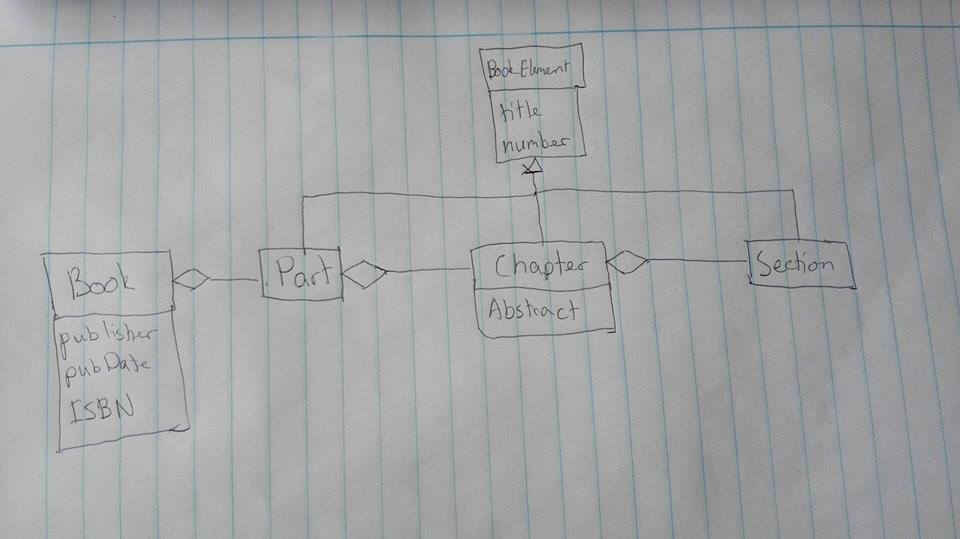
\includegraphics[scale=.5]{OOSE210.jpg} {\footnotesize OOSE 2.10}

\subsection{OOSE 5.3}
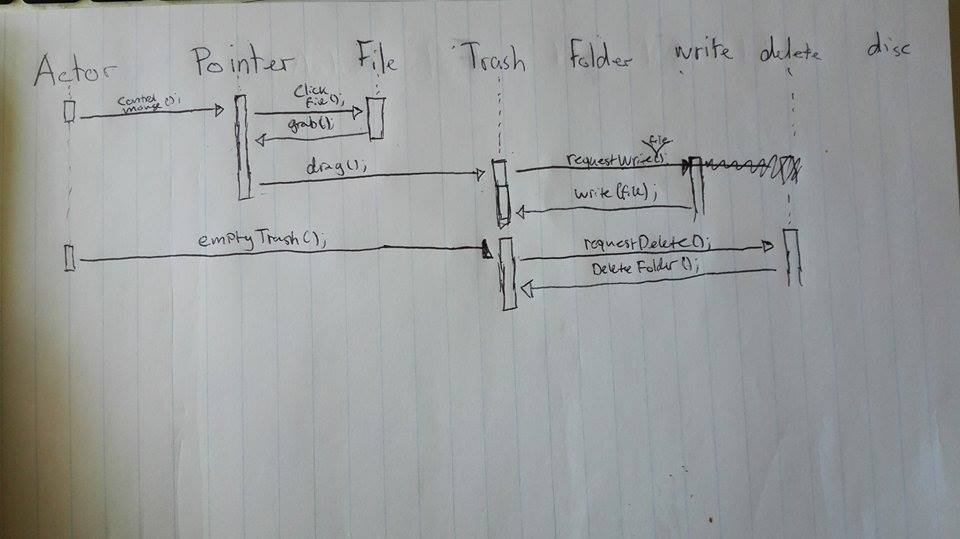
\includegraphics[scale=.5]{OOSE53.jpg} {\footnotesize OOSE 5.3}

\subsection{OOSE 7.1}



\end{document}

